% chktex-file 44
\section{Экспериментальная часть}
\subsection{Описание установки}
Рентгенографические эксперименты проводились на монокристальном дифрактометре Bruker D8 Venture (см. рисунок~\ref{fig:D8_photo}).
Его оборудование и характеристики:
\begin{itemize}
    \item Микрофокусная трубка Incoatec $I \mu S \ 3.0$
    \begin{itemize}
        \item $\text{Cu} K\alpha$ и $\text{Mo} K\alpha$ излучение
        \item Монохроматизация и коллимация с помощью многослойных зеркал Монтеля
        \item Диаметр пучка $110\unit{мкм}$
        \item Расходимость $0.3\degree$
    \end{itemize}
    \item Двумерный детектором PHOTON III
    \begin{itemize}
        \item CMOS-технология матрицы
        \item Разрешение $768 \times 1024$ пикселей
        \item Размер пикселя $135 \times 135\unit{мкм}^2$
        \item Ручная установка расстояния до образца
    \end{itemize}
    \item Трехкружный гониометр FIXED-CHI
    \begin{itemize}
        \item Гониометр использует эйлерову геометрию
        \item Автоматическая регулировка углов $\varphi$ и $\omega$ для образца и $2\theta_D$ для детектора
        \item Угол $\chi$ фиксирован и равен $54.7112\degree$
        \item Воспроизводимость установки углов $0.0001\degree$
        \item Точность установки углов $0.004\degree$\footnote{Паспортная точность установки углов не указана, но согласно результатам измерения эталонного образца на порошковом дифрактометре Bruker D8 Advance, оснащенном аналогичным гониометром, она не хуже $0.005\degree$.}
    \end{itemize}
    \item Температурная приставка Oxford Cryostream 800Plus
    \begin{itemize}
            \item Стабильность поддержания температуры $0.2\unit{К}$
    \end{itemize}
    \item Управление прибором средствами программного пакета APEX3~\cite{Bruker:2019}
\end{itemize}

\begin{figure}[ht!]
    \centering
    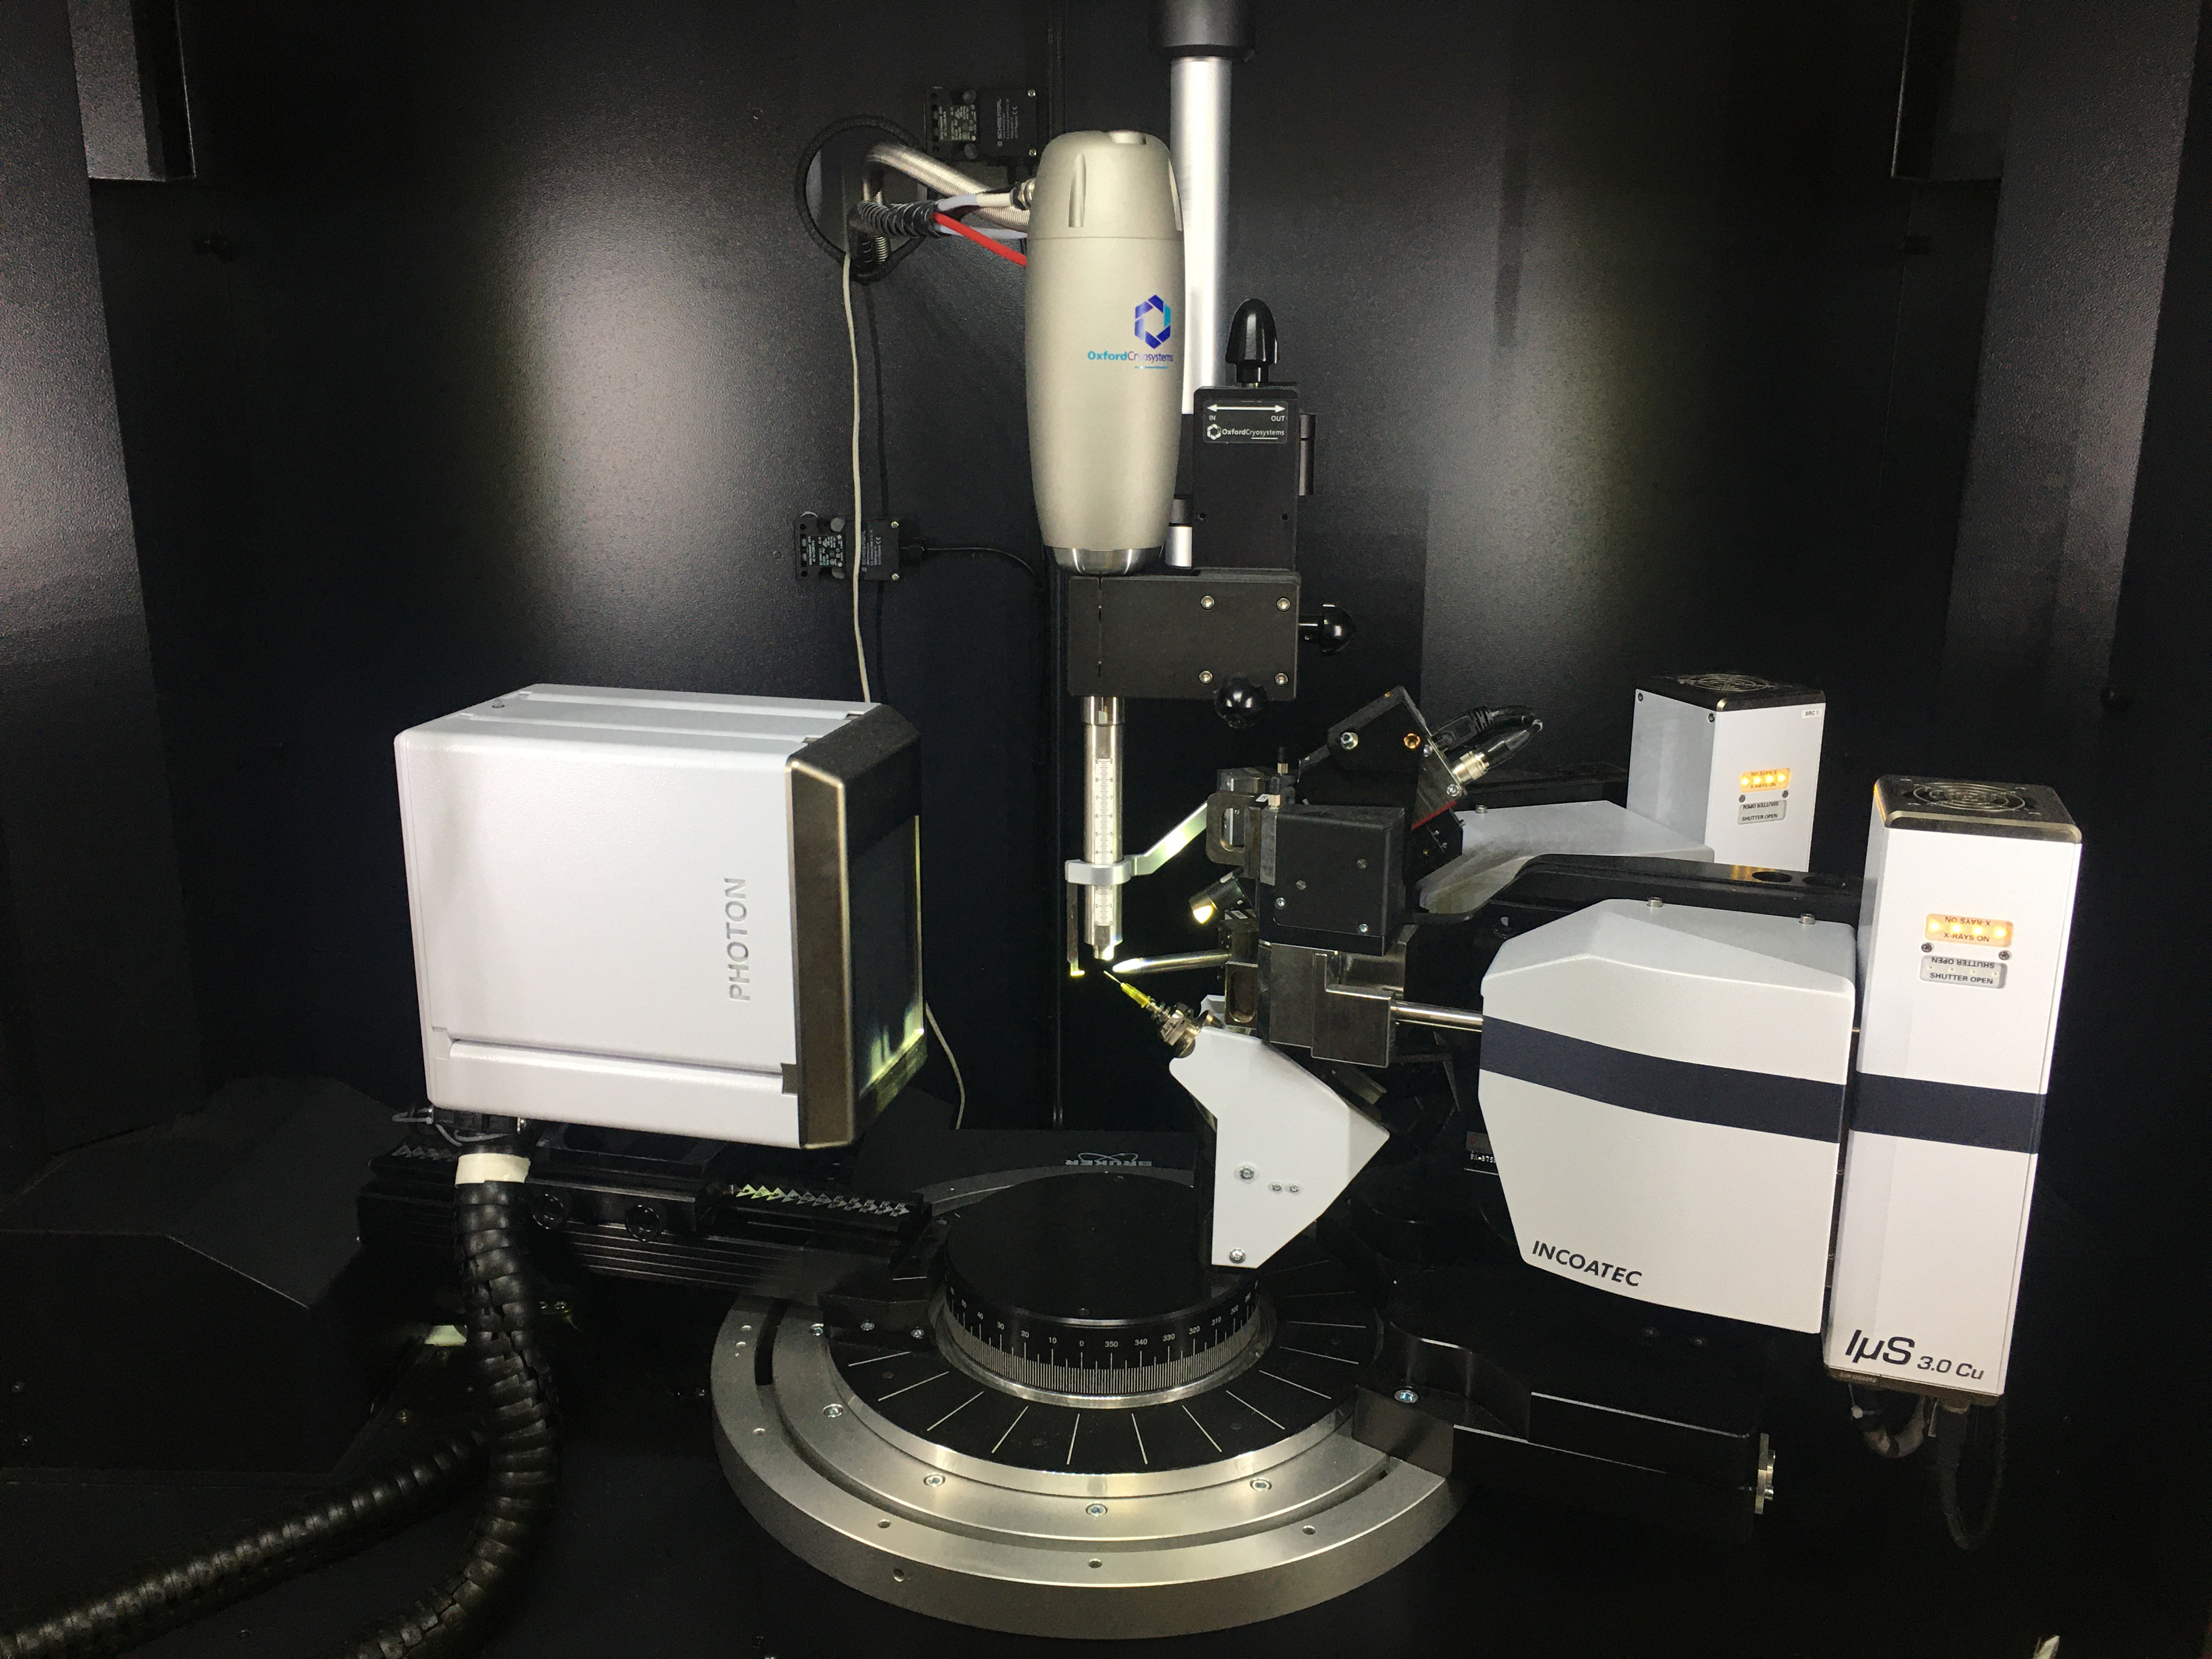
\includegraphics[width=0.8\textwidth]{d8_3.jpeg}
    \caption{Фотография установки}%
    \label{fig:D8_photo}
\end{figure}

\subsection{Исследуемые образцы}

Все изученные монокристаллы имели линейные размеры $\approx50\unit{мкм}$.
Монокристалл Si являлся осколком кристалла, который ранее был исследован на однокристальном спектрометре: $a_\text{Si} = 5.430933 (12)\unit{\AA}$~\cite{Lisoivan:1982}.
Однако, надо учесть, что это значение было вычислено исходя из $\lambda \text{Cu} K\alpha_1 = 1.540562\unit{\AA}$.
При использовании рекомендованной в настоящее время длины волны $\lambda \text{Cu} K\alpha_1 = 1.5405929\unit{\AA}$~\cite{Holzer:1997}, $a_\text{Si} = 5.431042(12)\unit{\AA}$.
Кристалл был смонтирован на гониометрической головке и тщательно сцентрирован (с поворотами по $\omega$ на $\pm 90\degree$). Для определения ориентации кристалла были проведены съемки трех серий $\varphi$-сканов шириной $0.5\degree$ при положениях детектора $2\theta_D = 0, \pm 45\degree$ (D = 70~мм).
Обработку фреймов проводили средствами APEX3 (процедуры: harvest, indexing, refinement), в результате был получен р4р-файл, содержащий информацию об ориентации кристалла относительно осей гониометра.
Аналогичная процедура была проведена с монокристаллом Ge.
Его ПЭЯ уточняли несколько раз методами однокристального спектрометра, многократных отражений и многолучевой дифракции: сводка данных приведена в~\cite{Lisoivan:1982}.
Значения $a_\text{Ge}$ лежат в интервале от $5.65776(2)\unit{\AA}$ до $5.657837(15)\unit{\AA}$, среднее значение $5.65779\unit{\AA}$ наиболее близко к $5.657772(10)\unit{\AA}$ [22].
Пересчет с использованием рекомендованного значения $\lambda \text{Cu} K\alpha_1 = 1.5405929\unit{\AA}$ приводит к $a_\text{Ge} = 5.657885\unit{\AA}$.

Монокристаллы \YEu{} получены методом роста из раствор-рас\-плава.
Продукт синтеза представлял собой мелкокристаллический порошок с размерами кристаллов от 0.2 до 1~мм.
Для исследования было отобрано 5 кристаллов с линейными размерами 20--40~мкм.

\subsection{Измерения в схеме Бонда}

Принципиальная схема эксперимента проведенного в схеме Бонда представлена на рис.~\ref{fig:bond}б.
В нашем случае наличие второго источника рентгеновского излучения ограничивает область доступных углов $2\theta_D$ значениями $\pm 97.5\degree$ (для $D = 128.5\unit{мм}$).
Второе ограничение связано со значительными геометрическими размерами детектора, что не дает блоку с установленной гониометрической головкой размещаться в определенных угловых интервалах.
По полученным р4р-файлам вычисляли углы $\varphi$ и $\omega$ для выведения рефлексов в отражающее положение на экваториальную плоскость.
Съемку рефлексов проводили в режиме $\omega$-сканирования угловых интервалов $\pm 2\degree$ относительно вычисленных значений $\omega$.
Такой интервал позволял зарегистрировать дублет полностью.
При съемке детектор устанавливали под углом $2\theta_D \approx 2\theta_{hkl}$, что обеспечивало регистрацию выбранного рефлекса центральной областью детектора.
Подробно методика описана в~\cite{Kudryavtsev:2024:YEu}.
Методику можно разделить на несколько этапов.

На первом этапе определяли ориентацию монокристалла относительно осей гониометра.
Такая съемка позволяет зарегистрировать существенную часть обратного пространства и провести качественное уточнение элементов матрицы ориентации для последующего вывода выбираемых рефлексов точно в отражающее положение на экваториальную окружность гониометра.
Кроме того, захват области дальних углов необходим для определения условий разрешения дублета $K\alpha$ и выяснения возможности уточнения ПЭЯ.
Обработку полученной серии фреймов проводили по программе APEX3.
В результате определяли предварительные значения ПЭЯ, дифракционный класс и ориентацию кристалла относительно осей гониометра (р4р-файл).
Этот этап соответствует первому этапу проведения РСтА.

Цель второго этапа --- поиск рефлексов, подходящих для измерения $d_{hkl}$.
В первую очередь мы рассматривали рефлексы с угловыми положениями $2\theta$ в узком интервале $\range{95\degree}{98\degree}$.
В случае эталонных монокристаллов (Si и Ge) структура известна, поэтому подходящие рефлексы были выбраны по теоретической дифрактограмме.
В общем случае, т.е. при неизвестной структуре, можно ориентироваться на предварительные значения ПЭЯ и дифракционный класс, установленный на первом этапе.
В случае Si и Ge для измерения ПЭЯ достаточно одного рефлекса, но для оценки уровня случайных ошибок взято большее количество.
Для поиска индексов кристаллографических плоскостей \hkl(h k l), которые могут быть выведены в отражающие положения при двух углах поворота детектора $2\theta_D$, была написана оригинальная программа James (язык Julia), доступная по ссылке https://github.com/m410y/James.jl.
Программа James использует информацию о текущей ориентации кристалла (р4р-файл) и вычисляет углы съемки $\varphi$ и $\omega$, при этом учитывая, что для записи рефлекса необходимо провести $\omega$-сканирование интервала $3-4\degree$.
Кроме этого, учитывается, что вывод в отражающее положение кристаллографической плоскости $(h k l)$, возможен при двух значениях $\omega$, число возможных ориентаций увеличивается вдвое (см. последний столбец табл. 1 Приложения).
Дополнительно программа сигнализирует о случаях, когда может быть использована и фриделевская пара \hkl(-h -k -l).
Съемка фриделевской пары позволяет по разнице значений координат $Y$ максимумов контролировать точность выведения рефлексов на экваториальную плоскость.
Некоторые дополнительные возможности программы James будут описаны далее.

На третьем этапе определяли общие условия проведения $\omega$-сканирования.
Для уменьшения ошибок, связанных с наклонами детектора, положение детектора задавали как $2\theta_D \approx 2\theta_{hkl}$.
При таком положении рефлекс фиксируется центральной областью детектора.
При выборе времени экспозиции ориентировались на получение интенсивности $K\alpha_1$-составляющей в максимуме $2 \cdot 10^4$ импульсов над фоном.
Время накопления фрейма в программе управления Bruker D8 Venture ограничено 10~мин, поэтому при необходимости, для достижения нужного уровня интенсивности, проводили несколько повторных съемок и далее суммировали фреймы средствами программы James. 
На четвертом этапе определяли координаты максимумов средствами программ Origin и James. Установлено, что результаты не отличаются.
Далее вычисляли разницу координат $X$ для двух симметричных положений детектора.
При переходе к углам дифракции рассчитывали угловые размеры пикселя $\gamma$, исходя из физических размеров пикселя ($135.3\unit{мкм}$) и выбранного $D$.
Контроль корректности такого расчета проводили по положениям $K\alpha_{1,2}$ составляющих согласно~\cite{Gromilov:2022}. 
Значение $2\theta_{hkl}$ вычисляли по формуле:
\begin{equation}\label{eq:bond2}
    2\theta_{hkl} = 2\theta_D + \gamma (X_- - X_+) / 2.
\end{equation}
При переходе к межплоскостному расстоянию $d$ использовали эталонное значение длины волны $\lambda \text{Cu} K\alpha_1 = 0.70931715(41)\unit{\AA}$.
Параметр элементарной кубической ячейки вычисляли по известной квадратичной форме: $1/d^2 = (h^2 + k^2 +l^2)/a^2$.
